\documentclass[border=12pt]{standalone}
\usepackage{amsmath, amssymb}
\usepackage{tikz}
\definecolor{ring0}{HTML}{0033CC}
\definecolor{ring1}{HTML}{0066FF}
\definecolor{ring2}{HTML}{0099FF}
\definecolor{ring3}{HTML}{00CCCC}
\definecolor{ring4}{HTML}{00CC66}
\definecolor{ring5}{HTML}{33CC00}
\definecolor{ring6}{HTML}{99CC00}
\definecolor{ring7}{HTML}{CCCC00}
\definecolor{ring8}{HTML}{FF9900}
\definecolor{ring9}{HTML}{FF6600}
\definecolor{ring10}{HTML}{FF3300}
\definecolor{ring11}{HTML}{CC0000}
\definecolor{gap0}{HTML}{E53935}
\definecolor{gap1}{HTML}{1E88E5}
\definecolor{gapfar}{HTML}{CCCCCC}
\begin{document}
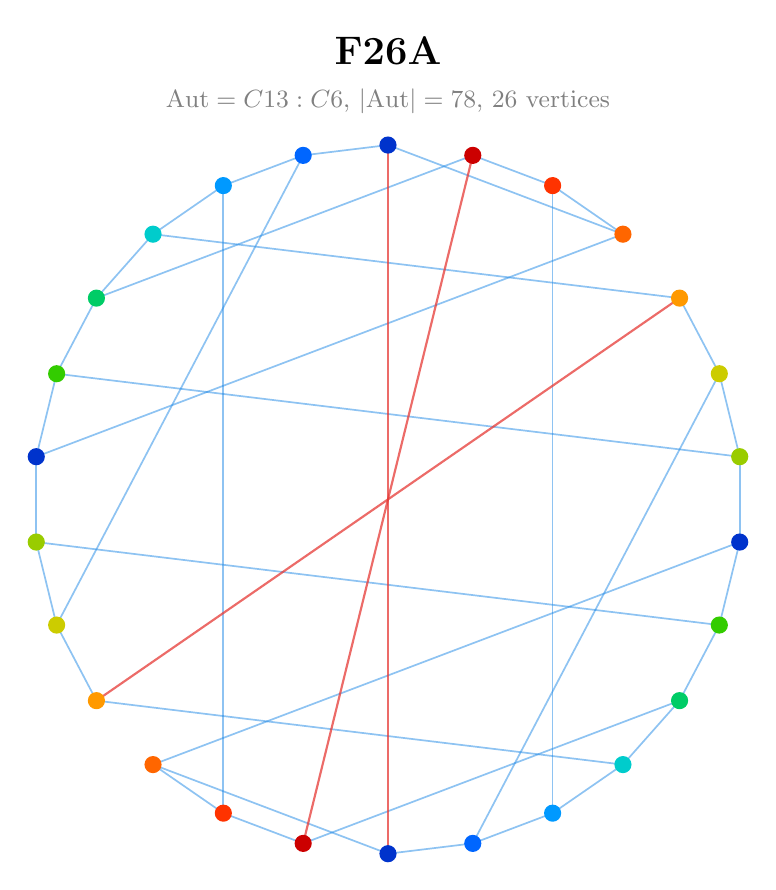
\begin{tikzpicture}
\node[font=\Large\bfseries] at (0, 5.70) {F26A};
\node[font=\small, text=gray] at (0, 5.05) {$\mathrm{Aut} = C13 : C6$, $|\mathrm{Aut}| = 78$, 26 vertices};
\draw[line width=0.62pt, gap1, opacity=0.50] (0.000, 4.500) -- (-1.077, 4.369);
\draw[line width=0.62pt, gap1, opacity=0.50] (0.000, 4.500) -- (2.984, 3.368);
\draw[line width=0.62pt, gap1, opacity=0.50] (-1.077, 4.369) -- (-2.091, 3.985);
\draw[line width=0.62pt, gap1, opacity=0.50] (-1.077, 4.369) -- (-4.208, -1.596);
\draw[line width=0.62pt, gap1, opacity=0.50] (-2.091, 3.985) -- (-2.984, 3.368);
\draw[line width=0.62pt, gap1, opacity=0.50] (-2.091, 3.985) -- (-2.091, -3.985);
\draw[line width=0.62pt, gap1, opacity=0.50] (-2.984, 3.368) -- (-3.703, 2.556);
\draw[line width=0.62pt, gap1, opacity=0.50] (-2.984, 3.368) -- (3.703, 2.556);
\draw[line width=0.62pt, gap1, opacity=0.50] (-3.703, 2.556) -- (-4.208, 1.596);
\draw[line width=0.62pt, gap1, opacity=0.50] (-3.703, 2.556) -- (1.077, 4.369);
\draw[line width=0.62pt, gap1, opacity=0.50] (-4.208, 1.596) -- (-4.467, 0.542);
\draw[line width=0.62pt, gap1, opacity=0.50] (-4.208, 1.596) -- (4.467, 0.542);
\draw[line width=0.62pt, gap1, opacity=0.50] (-4.467, 0.542) -- (-4.467, -0.542);
\draw[line width=0.62pt, gap1, opacity=0.50] (-4.467, 0.542) -- (2.984, 3.368);
\draw[line width=0.62pt, gap1, opacity=0.50] (-4.467, -0.542) -- (-4.208, -1.596);
\draw[line width=0.62pt, gap1, opacity=0.50] (-4.467, -0.542) -- (4.208, -1.596);
\draw[line width=0.62pt, gap1, opacity=0.50] (-4.208, -1.596) -- (-3.703, -2.556);
\draw[line width=0.62pt, gap1, opacity=0.50] (-3.703, -2.556) -- (2.984, -3.368);
\draw[line width=0.62pt, gap1, opacity=0.50] (3.703, 2.556) -- (4.208, 1.596);
\draw[line width=0.62pt, gap1, opacity=0.50] (4.208, 1.596) -- (4.467, 0.542);
\draw[line width=0.62pt, gap1, opacity=0.50] (4.208, 1.596) -- (1.077, -4.369);
\draw[line width=0.62pt, gap1, opacity=0.50] (4.467, 0.542) -- (4.467, -0.542);
\draw[line width=0.62pt, gap1, opacity=0.50] (4.467, -0.542) -- (4.208, -1.596);
\draw[line width=0.62pt, gap1, opacity=0.50] (4.467, -0.542) -- (-2.984, -3.368);
\draw[line width=0.62pt, gap1, opacity=0.50] (4.208, -1.596) -- (3.703, -2.556);
\draw[line width=0.62pt, gap1, opacity=0.50] (3.703, -2.556) -- (2.984, -3.368);
\draw[line width=0.62pt, gap1, opacity=0.50] (3.703, -2.556) -- (-1.077, -4.369);
\draw[line width=0.62pt, gap1, opacity=0.50] (2.984, -3.368) -- (2.091, -3.985);
\draw[line width=0.62pt, gap1, opacity=0.50] (2.091, -3.985) -- (1.077, -4.369);
\draw[line width=0.62pt, gap1, opacity=0.50] (2.091, -3.985) -- (2.091, 3.985);
\draw[line width=0.62pt, gap1, opacity=0.50] (1.077, -4.369) -- (-0.000, -4.500);
\draw[line width=0.62pt, gap1, opacity=0.50] (-0.000, -4.500) -- (-2.984, -3.368);
\draw[line width=0.62pt, gap1, opacity=0.50] (-2.984, -3.368) -- (-2.091, -3.985);
\draw[line width=0.62pt, gap1, opacity=0.50] (-2.091, -3.985) -- (-1.077, -4.369);
\draw[line width=0.62pt, gap1, opacity=0.50] (1.077, 4.369) -- (2.091, 3.985);
\draw[line width=0.62pt, gap1, opacity=0.50] (2.091, 3.985) -- (2.984, 3.368);
\draw[line width=0.78pt, gap0, opacity=0.75] (0.000, 4.500) -- (-0.000, -4.500);
\draw[line width=0.78pt, gap0, opacity=0.75] (-3.703, -2.556) -- (3.703, 2.556);
\draw[line width=0.78pt, gap0, opacity=0.75] (-1.077, -4.369) -- (1.077, 4.369);
\fill[ring0] (0.000, 4.500) circle (3.1pt);
\fill[ring1] (-1.077, 4.369) circle (3.1pt);
\fill[ring2] (-2.091, 3.985) circle (3.1pt);
\fill[ring3] (-2.984, 3.368) circle (3.1pt);
\fill[ring4] (-3.703, 2.556) circle (3.1pt);
\fill[ring5] (-4.208, 1.596) circle (3.1pt);
\fill[ring0] (-4.467, 0.542) circle (3.1pt);
\fill[ring6] (-4.467, -0.542) circle (3.1pt);
\fill[ring7] (-4.208, -1.596) circle (3.1pt);
\fill[ring8] (-3.703, -2.556) circle (3.1pt);
\fill[ring8] (3.703, 2.556) circle (3.1pt);
\fill[ring7] (4.208, 1.596) circle (3.1pt);
\fill[ring6] (4.467, 0.542) circle (3.1pt);
\fill[ring0] (4.467, -0.542) circle (3.1pt);
\fill[ring5] (4.208, -1.596) circle (3.1pt);
\fill[ring4] (3.703, -2.556) circle (3.1pt);
\fill[ring3] (2.984, -3.368) circle (3.1pt);
\fill[ring2] (2.091, -3.985) circle (3.1pt);
\fill[ring1] (1.077, -4.369) circle (3.1pt);
\fill[ring0] (-0.000, -4.500) circle (3.1pt);
\fill[ring9] (-2.984, -3.368) circle (3.1pt);
\fill[ring10] (-2.091, -3.985) circle (3.1pt);
\fill[ring11] (-1.077, -4.369) circle (3.1pt);
\fill[ring11] (1.077, 4.369) circle (3.1pt);
\fill[ring10] (2.091, 3.985) circle (3.1pt);
\fill[ring9] (2.984, 3.368) circle (3.1pt);
\end{tikzpicture}
\end{document}